\documentclass{beamer}
\usepackage[ngerman]{babel}			%Deutsche Umlaute und Umbrüche
\usepackage[utf8]{inputenc}			%utf8 Kodierung
\usepackage{amsmath, amsfonts, amssymb, ulem, epstopdf} %Mathepackete schaden nie
\usetheme{Dresden}
\usecolortheme{beaver}
\usefonttheme{professionalfonts}
\title[TODO]{TODO}
\subtitle{Architectural Document}
\author[C. Stricker\and A. Klein\and D. Klopp\and M. Vieth]{Christian Stricker\and Alisha Klein\and David Klopp\and Markus Vieth}
\date[\today]{\today}
\subject{Software engineering}
\newcommand{\btVFill}{\vskip0pt plus 1filll}
\setcounter{tocdepth}{2}
%Link zum Beamer-Userguid: ftp://ftp.dante.de/tex-archive/macros/latex/contrib/beamer/doc/beameruserguide.pdf
\begin{document}
	
	\frame{
		\titlepage
	}
	\setbeamertemplate{footline}[frame number]
	
	\frame[label=IV]{
		\frametitle{Inhaltsverzeichnis}
		\tableofcontents
		[pausesections]
	}
	
	\section{Client}
	\begin{frame}{Factory}
		\begin{figure}
			\centering
			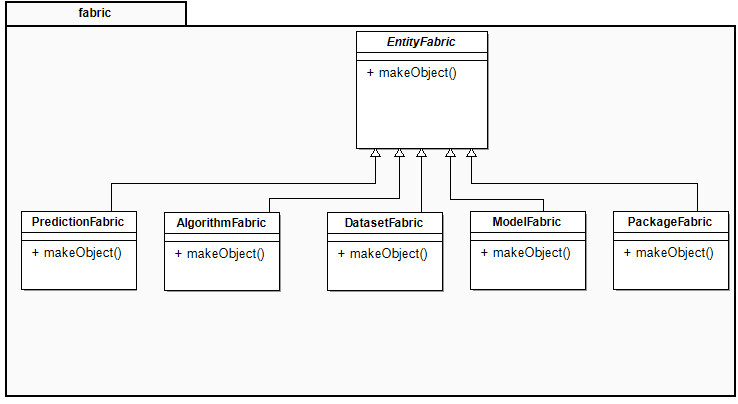
\includegraphics[width=\linewidth]{Grafik/Klassendiagramme/fabrik}
			\caption{Fabrik-Pattern}
			\label{fig:Fabrik}
		\end{figure}
	\end{frame}
	
	\begin{frame}{Servlet}
		\begin{figure}
			\centering
			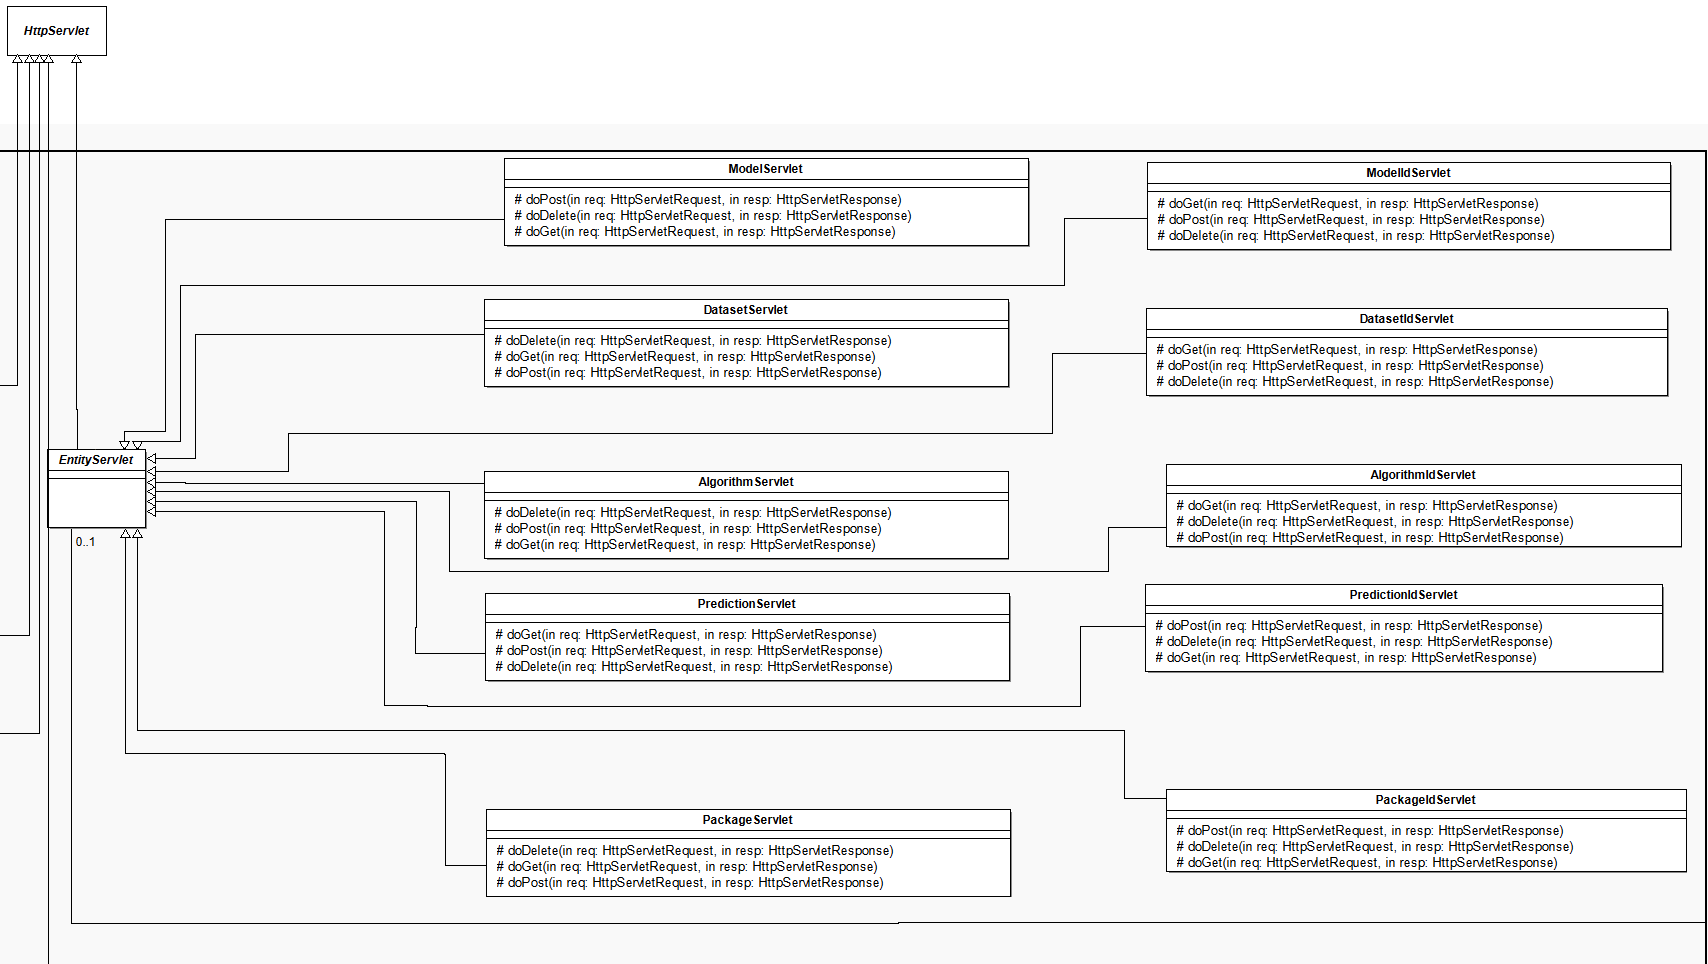
\includegraphics[width=\linewidth]{Grafik/Klassendiagramme/Servlet1}
			\caption{Servlets1}
			\label{fig:Servlets1}
		\end{figure}
	\end{frame}	
	\begin{frame}{Servlet}
		\begin{figure}
			\centering
			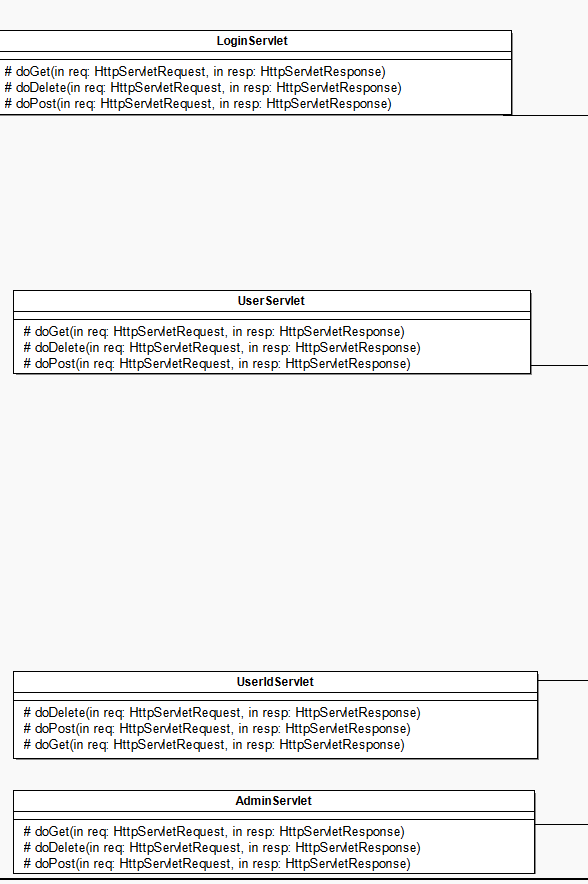
\includegraphics[height=0.8\textheight]{Grafik/Klassendiagramme/Servlet2}
			\caption{Servlets2}
			\label{fig:Servlets2}
		\end{figure}
	\end{frame}
	
	\section{Server}
	\begin{frame}{Adapter}
		\begin{figure}
			\hspace*{-35pt}
			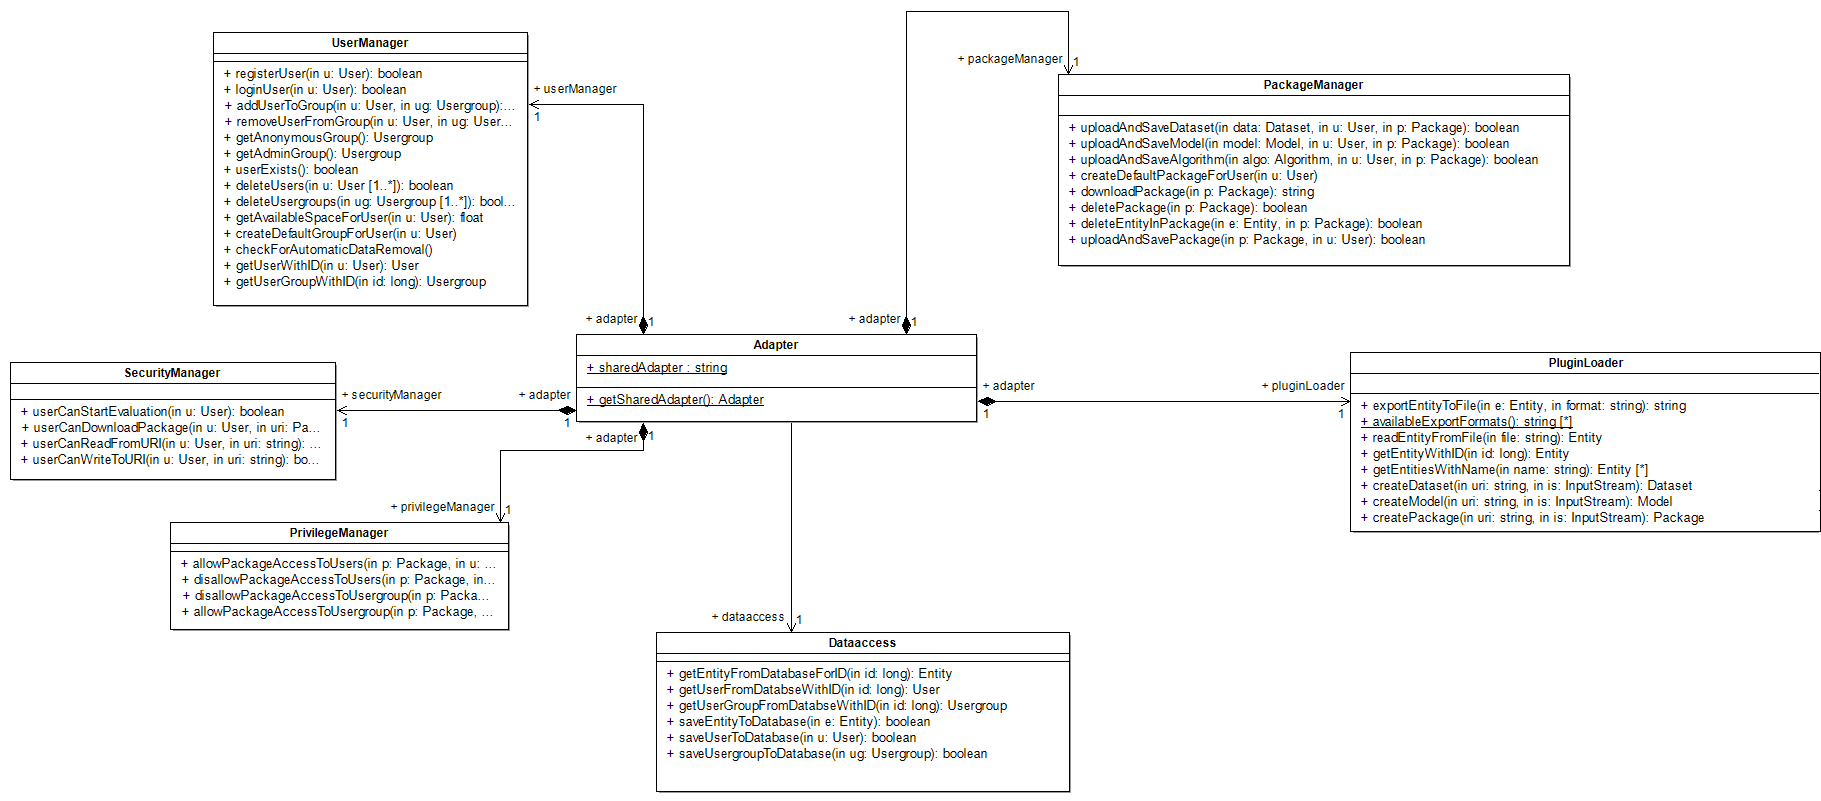
\includegraphics[width=1.25\linewidth]{Grafik/Klassendiagramme/adapter}
			\caption{Adapter}
			\label{fig:Adapter}
		\end{figure}
	\end{frame}
	\begin{frame}{WEKA}
		\begin{figure}
			%\hspace*{-35pt}
			\centering
			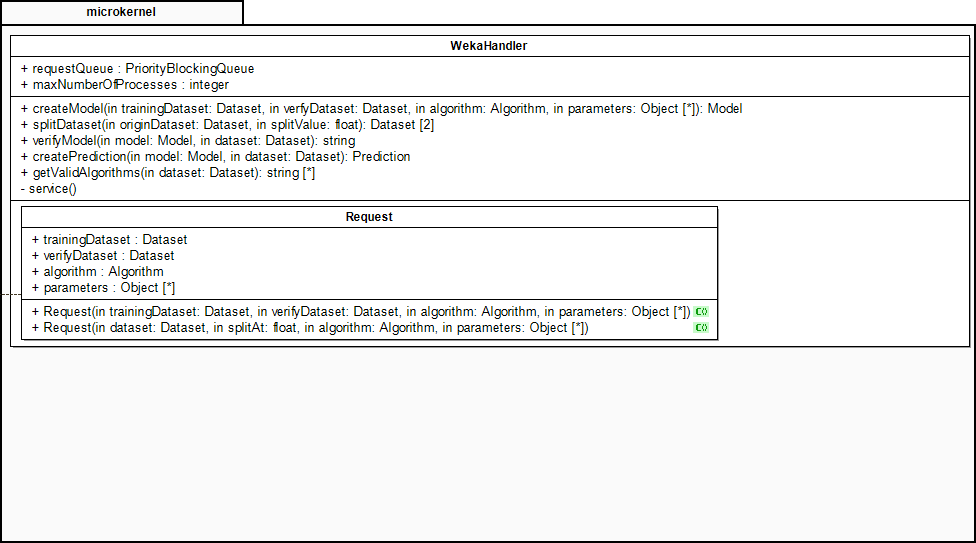
\includegraphics[width=1\linewidth]{Grafik/Klassendiagramme/Weka}
			\caption{WEKA}
			\label{fig:WEKA}
		\end{figure}
	\end{frame}
	
	
		\section{Sequenzdiagramme}
		\begin{frame}{Modelerstellung}
			\begin{figure}
				\hspace*{-30pt}
				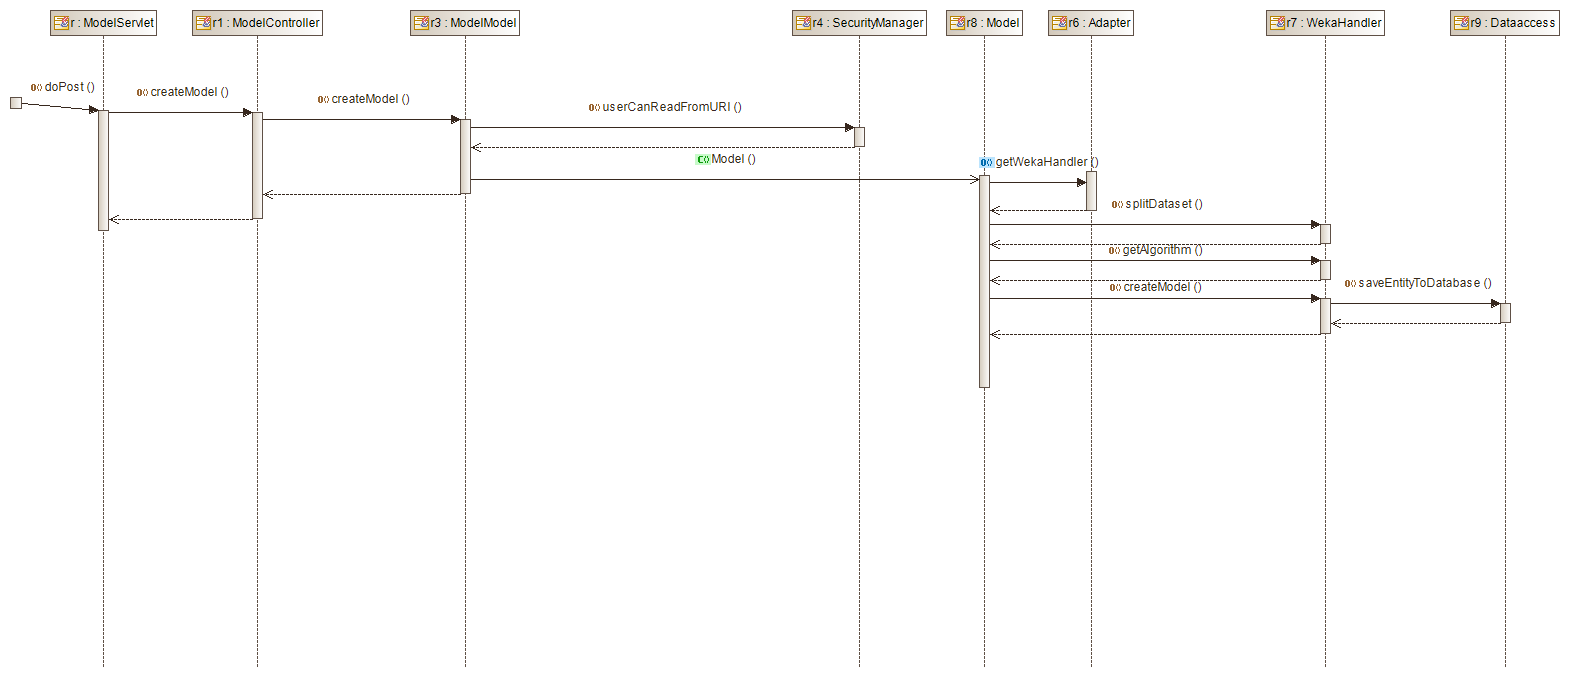
\includegraphics[width=1.175\linewidth]{Grafik/Sequenzdiagramme/Modelerstellung}
				\caption{Modelerstellung}
				\label{fig:Modelerstellung}
			\end{figure}
		\end{frame}
		
\end{document}